% !TeX spellcheck = pl_PL
\chapter{Testowanie i uruchamianie}
\section{Testowanie wyznaczania maksymalnego przepływu}\label{sec:testNetwork}
W ramach testowania poprawności działania algorytmów wyznaczania maksymalnego przepływu zostało utworzonych kilka podręcznikowych sieci przepływowych, które były modelem do testowania algorytmów.
\begin{enumerate}
	\item Na rys. \ref{fig:test1} znajduje się sieć przepływowa, w której suma przepływów netto wychodzących ze źródła jest mniejsza niż suma przepływów netto wchodzących do ujścia, $ \sum_{v\in V}{c(s,v)} < \sum_{v\in V}{c(v,t)} $. Łuki pośredniczące posiadają wystarczająco dużą przepustowość aby móc przenieść cały przepływ wychodzący ze źródła do krawędzi wchodzących do ujścia. Test oczekuje, że maksymalny przepływ sieci $ |f| $ będzie mieć wartość nie większą niż $ \sum_{v\in V}{c(s,v)}=10+10=20 $.
	\item Na rys. \ref{fig:test2} znajduje się sieć o podobnej strukturze, tym razem $ \sum_{v\in V}{c(s,v)} > \sum_{v\in V}{c(v,t)} $. Łuki pośredniczące tak samo są w stanie przenieść sumę przepływów wychodzących ze źródła do krawędzi wchodzących do ujścia, więc test oczekuje, że przepływ sieci $ |f| $ będzie mieć wartość nie większą niż $ \sum_{v\in V}{c(v,t)}=30+10=40 $.
	\item Na rys. \ref{fig:test3} przedstawiono strukturę w której $ \sum_{v\in V}{c(s,v)} = \sum_{v\in V}{c(v,t)} $, ale łuki pośredniczące nie są w stanie przenieść całego przepływu. Dla łuku $ (s, 2) $, gdzie $ c(s,2)=40 $, jedyna ścieżka do ujścia prowadzi przez $ s\rightarrow2\rightarrow4\rightarrow t $, gdzie przepustowość residualna tej ścieżki jest równa $ c(2,4)=10 $. Z kolei dla łuku $ (s, 3) $, gdzie $ c(s,3)=30 $, ścieżki prowadzące do ujścia (przy założeniu, że łuk $ (2,4) $ został nasycony w poprzednim kroku) to $ s\rightarrow3\rightarrow4\rightarrow t $ o przepustowości residualnej równej $ c(3,4)=20 $ oraz $ s\rightarrow3\rightarrow5\rightarrow t $ o przepustowości residualnej równej $ c(3,5)=10 $. Podsumowując, test oczekuje, że przepływ sieci $ |f| $ będzie mieć wartość nie większą niż suma przepustowości residualnych tych trzech ścieżek, $ 10+20+10=40 $.
\end{enumerate}
Wszystkie przypadki testowe zostały sprawdzone poprzez statyczne wprowadzenie sieci do aplikacji oraz ręczne uruchomienie algorytmów. Wyniki zostały przedstawione w tabelach \ref{table:test1}, \ref{table:test2} i \ref{table:test3}. Obliczenia zostały wykonane na komputerze z procesorem \textit{Intel Celeron G530 2 x 2.4 GHz}, 6 GB pamięci RAM i systemem \textit{Windows 7 x64}.
\section{Wyniki}
Zgodnie z danymi przedstawionymi w tabelach \ref{table:test1}, \ref{table:test2} i \ref{table:test3} we wszystkich sieciach przepływowych został obliczony maksymalny przepływ, który spełniał teoretyczne założenia opisane w rozdziale \ref{sec:testNetwork}. Z kolumny \textit{czas wykonania} wynika, że najefektywniejszym algorytmem jest algorytm MKM, który dla najbardziej trudnego przypadku (zakończenie algorytmu przez zauważenie zapełnienia łuków pośrednich) wykonał się zdecydowanie najszybciej, ponad dwa razy szybciej niż algorytm Forda-Fulkersona. Algorytm Dinica zajmuje drugie miejsce, jest o wiele efektywniejszy niż algorytm Forda-Fulkersona, ale trochę wolniejszy niż MKM. Z kolei dla pierwszej sieci czas wykonania algorytmów jest w przybliżeniu taki sam, ze wskazaniem na algorytm Forda-Fulkersona jako najlepszy. Stało się tak dlatego, że w tym przypadku łuki wychodzące ze źródła szybko się nasycają i algorytm Forda-Fulkersona wykonuje się trochę szybciej, ponieważ tworzy mniej złożone struktury.
\begin{figure}
	\centering
	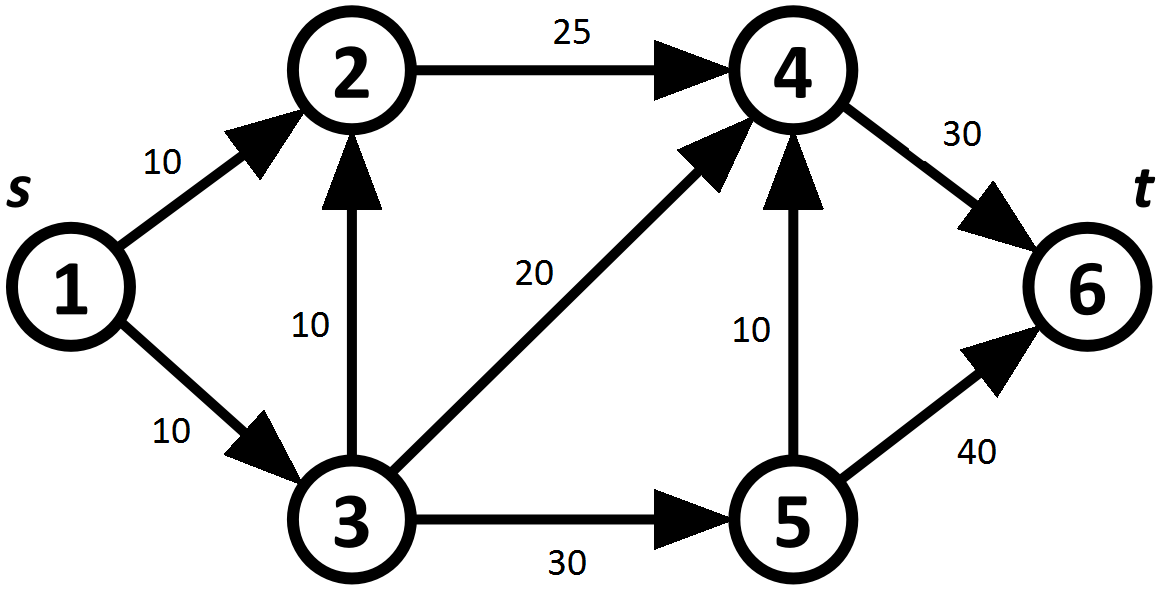
\includegraphics[width=0.5\textwidth]{./img/test1}
	\caption{Sieć z ograniczeniem przepływu u źródła}
	\label{fig:test1}
\end{figure}
\begin{figure}
	\centering
	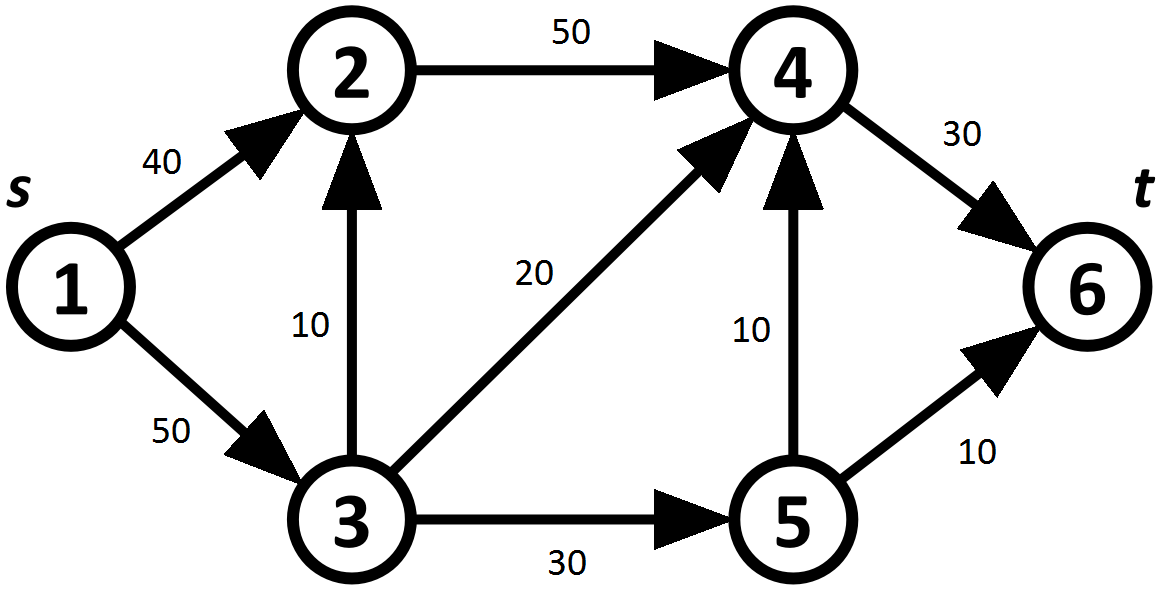
\includegraphics[width=0.5\textwidth]{./img/test2}
	\caption{Sieć z ograniczeniem przepływu u ujścia}
	\label{fig:test2}
\end{figure}
\begin{figure}
	\centering
	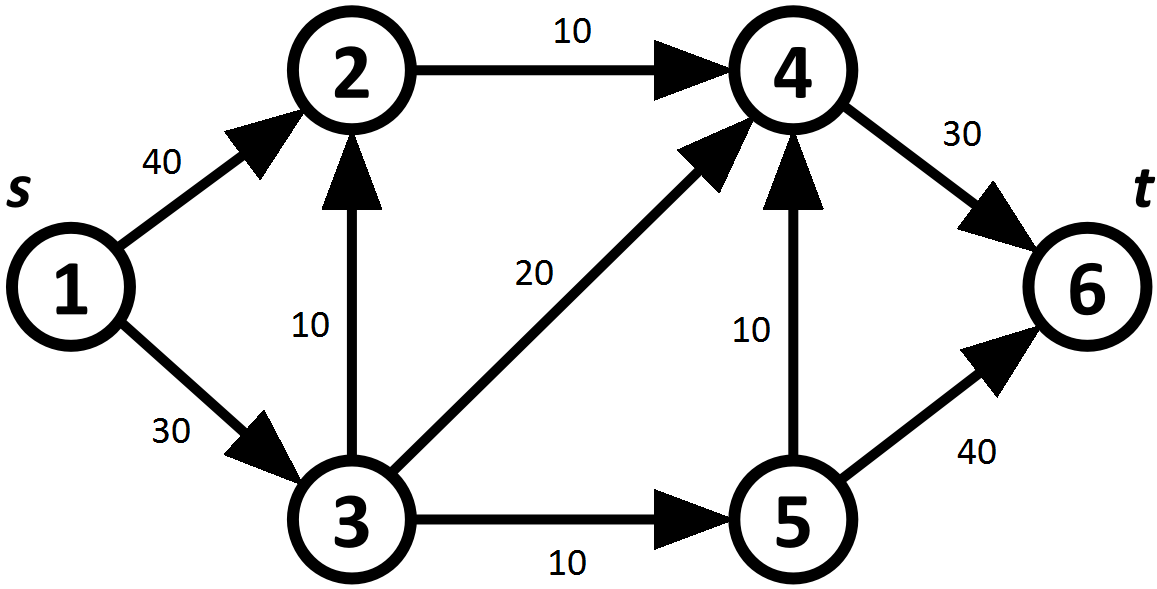
\includegraphics[width=0.5\textwidth]{./img/test3}
	\caption{Sieć z ograniczeniem przepływu między źródłem, a ujściem}
	\label{fig:test3}
\end{figure}
\begin{table}
	\centering
	\begin{tabular}{|c|c|c|c|}\hline
		\textbf{Algorytm} & \textbf{Maksymalny przepływ} & \textbf{Czy prawidłowy?} & \textbf{Czas wykonania} [ms] \\[1pt]\hline
		Forda-Fulkersona        &     20                &    Tak             &      132          \\[1pt]
		Dinica        &       20              &      Tak           &     136           \\[1pt]
		MKM        &      20               &       Tak          &        137        \\\hline
	\end{tabular}
	\caption{Wyniki testu dla sieci na rys. \ref{fig:test1}}
	\label{table:test1}
\end{table}
\begin{table}
	\centering
	\begin{tabular}{|c|c|c|c|}\hline
		\textbf{Algorytm} & \textbf{Maksymalny przepływ} & \textbf{Czy prawidłowy?} & \textbf{Czas wykonania} [ms] \\[1pt]\hline
		Forda-Fulkersona        &     40                &    Tak             &      221          \\[1pt]
		Dinica        &       40              &      Tak           &     149           \\[1pt]
		MKM        &      40               &       Tak          &        144        \\\hline
	\end{tabular}
	\caption{Wyniki testu dla sieci na rys. \ref{fig:test2}}
	\label{table:test2}
\end{table}
\begin{table}
	\centering
	\begin{tabular}{|c|c|c|c|}\hline
		\textbf{Algorytm} & \textbf{Maksymalny przepływ} & \textbf{Czy prawidłowy?} & \textbf{Czas wykonania} [ms] \\[1pt]\hline
		Forda-Fulkersona        &     40                &    Tak             &      435          \\[1pt]
		Dinica        &       40              &      Tak           &     250           \\[1pt]
		MKM        &      40               &       Tak          &        201        \\\hline
	\end{tabular}
	\caption{Wyniki testu dla sieci na rys. \ref{fig:test3}}
	\label{table:test3}
\end{table}